% arara: xelatex: { synctex: true, action: nonstopmode, options: "-halt-on-error -shell-escape" }
% arara: biber
% arara: biber
% arara: makeglossaries
% arara: xelatex: { synctex: true, action: nonstopmode, options: "-halt-on-error -shell-escape" }
% arara: clean: { files: [ comp3091-mattbell.aux, comp3091-mattbell.bbl, comp3091-mattbell.bcf, comp3091-mattbell.blg, comp3091-mattbell.log, comp3091-mattbell.out, comp3091-mattbell.synctex.gz, comp3091-mattbell.run.xml ] }
\documentclass[a4paper]{report}
\usepackage[utf8]{inputenc}
\usepackage{setspace}
\usepackage{xargs}
%\usepackage{subfigure}

\usepackage[backend=biber]{biblatex}
\addbibresource{report.bib}
\usepackage{fontspec}
\usepackage{titlesec}
\usepackage[dvipsnames]{xcolor}
\usepackage[acronym,toc,section]{glossaries}
\renewcommand*{\glsclearpage}{}
\makeglossaries

\newglossaryentry{lorawan}
{
  name=LoRaWAN,
  description={Wireless data transmission standard designed for long range communication at low power, at the cost of a lower data transmission rate}
}

\newglossaryentry{6lowpan}
{
  name=6LoWPAN,
  description={Short-range wireless data transmission standard. Short for ``IPv6 over LOw Power Wireless Personal Area Networks''; alternative to protocols like Bluetooth and Zigbee}
}

\newglossaryentry{contiki}
{
  name={Contiki},
  description={A Real-Time Operating System (RTOS) designed specifically for the Internet of Things. Contains a full network stack and can run on a minimal system, with lower power consumption}
}

\newglossaryentry{mips}
{
  name={MIPS},
  description={Multiprocessor without Interlocked Pipeline Stages, a type of
  processor architecture}
}

\newglossaryentry{mikrobus}
{
  name={mikroBUS},
  description={Bus standard for integrating IoT sensors onto
  development boards. Contains pins for SPI, analog data transmission, power,
  and an interrupt pin}
}

\newglossaryentry{opcode}
{
  name={opcode},
  description={Short for operation code, a command or instruction that may be part of a device's instruction list}
}

\newglossaryentry{overfit}
{
  name=overfit,
  description={Where a statistical or machine learning model is adjusted so
  that it works extremely well on training data, but does not work so well on
  non-training data.}
}
\newacronym{iot}{IoT}{Internet of Things}
\newacronym{api}{API}{Application Programming Interface}
\newacronym{rtos}{RTOS}{Real-Time Operating System}
\newacronym{io}{I/O}{Input/output}
\newacronym{ipv6}{IPv6}{Internet Protocol version 6}
\newacronym{ipv4}{IPv4}{Internet Protocol version 4}
\newacronym{json}{JSON}{JavaScript Object Notation}
\newacronym{tcp}{TCP}{Transmission Control Protocol}
\newacronym{udp}{UDP}{User Data Protocol}
\newacronym{spi}{SPI}{Serial Peripheral Interface bus}
\newacronym{http}{HTTP}{Hyper-Text Transfer Protocol}
\newacronym{bdd}{BDD}{Behaviour-Driven Development}
\newacronym{tdd}{TDD}{Test-Driven Development}
\newacronym{ghz}{GHz}{Gigahertz}
\newacronym{ap}{AP}{Access Point}
\newacronym{ssh}{SSH}{Secure Shell}
\newacronym{mcu}{MCU}{Microcontroller Unit}
\newacronym{rgb}{RGB}{Red, Green, Blue}
\newacronym{cnn}{CNN}{Convolutional Neural Network}
\definecolor{colorDoc}{HTML}{333333}

\usepackage{minted}
\usemintedstyle{pastie}

% https://tex.stackexchange.com/a/178806
\usepackage[colorinlistoftodos,prependcaption,textsize=tiny]{todonotes}
\newcommandx{\unsure}[2][1=]{\todo[linecolor=red,backgroundcolor=red!25,bordercolor=red,#1]{#2}}
\newcommandx{\change}[2][1=]{\todo[linecolor=blue,backgroundcolor=blue!25,bordercolor=blue,#1]{#2}}
\newcommandx{\info}[2][1=]{\todo[linecolor=OliveGreen,backgroundcolor=OliveGreen!25,bordercolor=OliveGreen,#1]{#2}}
\newcommandx{\improvement}[2][1=]{\todo[linecolor=Plum,backgroundcolor=Plum!25,bordercolor=Plum,#1]{#2}}
\newcommandx{\thiswillnotshow}[2][1=]{\todo[disable,#1]{#2}}

\newfontfamily\headingfont[]{Apercu}
\setmonofont[Color=colorDoc]{Apercu Mono}
% \setmainfont[Color=colorDoc]{Apercu}
\titleformat
{\chapter} % command
[display] % shape
{\bfseries\huge\headingfont} % format
{\chaptername \ \thechapter} % label
{0.5ex} % sep
{
  \Huge
} % before-code
\titleformat*{\section}{\LARGE\bfseries\headingfont}
\titleformat*{\subsection}{\Large\bfseries\headingfont}
\titleformat*{\subsubsection}{\large\bfseries\headingfont}
\defbibheading{bibempty}{}
% \renewcommand{\maketitlehooka}{\headingfont}

\pagestyle{plain}
\usepackage{amssymb,graphicx,color}
\graphicspath{{images/}}
\usepackage{amsfonts}
\usepackage{latexsym}
\usepackage{a4wide}
\usepackage{amsmath}

\newtheorem{theorem}{THEOREM}
\newtheorem{lemma}[theorem]{LEMMA}
\newtheorem{corollary}[theorem]{COROLLARY}
\newtheorem{proposition}[theorem]{PROPOSITION}
\newtheorem{remark}[theorem]{REMARK}
\newtheorem{definition}[theorem]{DEFINITION}
\newtheorem{fact}[theorem]{FACT}

\newtheorem{problem}[theorem]{PROBLEM}
\newtheorem{exercise}[theorem]{EXERCISE}
\def \set#1{\{#1\} }

\newenvironment{proof}{
PROOF:
\begin{quotation}}{
$\Box$ \end{quotation}}



\newcommand{\nats}{\mbox{\( \mathbb N \)}}
\newcommand{\rat}{\mbox{\(\mathbb Q\)}}
\newcommand{\rats}{\mbox{\(\mathbb Q\)}}
\newcommand{\reals}{\mbox{\(\mathbb R\)}}
\newcommand{\ints}{\mbox{\(\mathbb Z\)}}

%%%%%%%%%%%%%%%%%%%%%%%%%%


\title{{\vspace{-14em} 
\includegraphics[scale=0.4]{ucl_logo.png}}\\
{{\Huge Tracking Wildlife Counts Using the Internet Of Things}}\\
% {\large Optional Subtitle}\\
}
\date{Submission date: Day Month Year}
\author{Matthew Bell\thanks{
{\bf Disclaimer:}
This report is submitted as part requirement for the Computer Science BSc at
UCL. It is substantially the result of my own work except where explicitly
indicated in the text.
The report may be freely copied and distributed provided the source is explicitly acknowledged.}
\\ 
\texttt{m.bell@cs.ucl.ac.uk}\\ \\
BSc Computer Science\\ \\
Supervisor: Dr Kevin Bryson}


\begin{document}
 
\onehalfspacing
\maketitle
\begin{abstract}
  Conservation experts, park rangers, and biologists frequently aim to try to
track the location and count of various species of animals for a number of
reasons, such as preventing illegal poaching and hunting, monitoring
biodiversity, or analysing migration patterns. This is, more often than not,
extremely time consuming, since researchers have to install camera traps with
motion sensing shutters, and manually look back through images to identify
and count the animals.

This project and report explores the possibility of using a low-power
computer with sensors, connected to a web server over a wireless Internet
connection (a paradigm frequently referred to as \textit{The \acrfull{iot}})
to automate this task to save researchers many hours of time when conducting
studies using camera traps.

The project also explores various methods in which species of animals could
be identified automatically using deep learning techniques, such as using
convolutional neural networks, with the constraint of having to operate on
remote, low-powered hardware with limited Internet connectivity.

The project proved to be a lot more difficult than first anticipated, thanks
to unforseen issues with the hardware being used, as well as difficulties in
developing a rigourous image classifier. However, it proved to be an
incredibly valuable learning experience, and provided the opportunity to work
in a problem domain that would not normally be possible in an undergraduate
computer science degree.
\end{abstract}

\listoftodos[To-Do (Delete Before Submission)]

\tableofcontents
\setcounter{page}{1}


\chapter{Introduction and background}

\section{Motivation and need}
Wildlife conservation experts constantly need to keep track of the location
and movements of wildlife for a number of reasons, including monitoring
species migration patterns and population
counts~\cite{karanth1995estimating}. Other options exist, like line transect
surveys (counting animals or traces of animals, like tracks and droppings) or
track surveys (physically visiting the area and counting animals); but in the
comparison study by Silveira et al~\parencite{silveira2003camera}, they found
that camera traps, despite their longer initial setup time and cost, ``can be
handled more easily and with relatively [lower] costs in a long term run''.

Based on this, it would be logical to assume that running costs and analysis
time could be reduced further by automating the classification of photos
taken by camera traps and sending the results back to a web server. This
would enable research teams to store, access, analyse and visualise wildlife
counts with ease, using an \acrfull{api} provided by the web service.

The biggest advantage of automating the classification stage of camera trap
studies is that it would save a lot of time after the main study has ended,
and results can be analysed as soon as possible.

\section{Requirements}

A list of requirements for the solution were reasonably easy to devise. Most
of the requirements are defined by the limits of the environments where this
system may be deployed, such as woodlands, grasslands, and national parks.

Most of the locations where this solution could be deployed may have very
limited cell network coverage, and definitely would not have WiFi
connectivity available. Therefore, the system would have to use
\gls{lorawan}, which has a theoretical range of up to twenty kilometres.
However, the lower data rate of \gls{lorawan} means that photos captured by
the camera traps would not be able to be sent back to a web server, so any
kind of image processing and classification would have to be performed
on-device.

Another limitation is the devices provided for the project. The main ``base
station'' device is the Creator Ci40 developer board, designed to ``allow
developers to rapidly create connected products''~\cite{creatorci40}. This
ability to rapidly prototype on the board, which has a MIPS-based processor
and runs the OpenWRT Linux distribution, means that, in theory, it is a
perfect match for this project. It also contains a WiFi radio, useful for
communicating with the device and debugging code on it during development,
and a \gls{6lowpan} radio, useful for communicating with nearby devices.

The sensor devices were also provided as part of the project. They each
consist of a sensor board integrated onto a \textit{MikroElektronika}
\gls{6lowpan} clicker board~\cite{mikroeclick}. These boards run a
\acrfull{rtos}, which allows the board to respond very quickly to changes in
sensor input, as well as run with a low power consumption (because of less
computation overhead) and the inclusion of a \gls{6lowpan} radio, to
communicate with the base station.

Another requirement arising from the intended deployment scenario is that the
system needs to be able to run on battery power, or indeed a low-voltage
power source, for a considerable amount of time. The intention of the project
is to reduce long-term study costs, and a need to replace sensor batteries
regularly would be failing this. Consequently, the system would have to rely
on hardware interrupts as much as possible, so that the devices can remain in
a ``sleep mode'' when they are not needed.

\subsection{Expected Outcomes And Deliverables}
Below is a list of the expected outcomes and deliverables specified at the
start of the project.

\begin{itemize}
    \item A program built for the Creator Ci40 prototyping board that can read
        in an image sent by the external camera module, and classify the types
        and counts of animals in the image, before sending this data to a base
        station via a LORA connection
    \item A program for the IR clicker device to detect movement and send a
        message to a nearby camera device
    \item A program for the camera device to take a photo when it receives a
        command via 6LoWPAN and send it to the Ci40 board
    \item A simple cloud service to store and display results received from the
        prototype boards
    \item A rigorous testing regime for as much code as possible
    \item (If possible) a real-life test of the system in an uncontrolled
        environment (i.e. a park or zoo)
\end{itemize}

\section{Research}

The next step after gathering these requirements from the supervisor was to
find existing research and solutions to similar problems. These papers,
articles and reports have been compiled below.

\subsection{Similar Projects, Papers and Articles}

\subsubsection{Towards Automatic Wild Animal Monitoring: Identification of
Animal Species in Camera-trap Images using Very Deep Convolutional Neural
Networks}
In this paper by Gómez et al~\cite{gomez2016towards}, a similar project is
detailed to this one, in which the authors create a \acrlong{cnn} using the
same Snapshot Serengeti~\cite{swanson2015snapshot} camera trap images. Their
model uses ``off-the-shelf'' features of their chosen framework, and acheived
a ``top-5'' accuracy of 88.9\%, which is significant when compared to the
crowdsourced classifications which obtained an accuracy of
96\%~\cite{swanson2015snapshot}.

\subsubsection{Automatically identifying, counting, and describing wild
animals in camera-trap images with deep learning}
This paper by Norouzzadeh et al~\cite{norouzzadehautomatically} is in a
similar tone to the paper published by Gómez et al~\cite{gomez2016towards}.
They use the same Snapshot Serengeti dataset, but manage an accuracy of
``over 93.8\%'', and can also ``ìdentify count and describe animals'' in the
images (identifying features like whether the animals are standing or not, if
they are moving or not, and so on). The authors conclude that they can ``save
99.3\% of the manual labour (over 17,000 hours) while performing at the same
96.6\% accuracy level of human volunteers'', and highlight the benefits of
having more labour time for other scientific activities.

\subsubsection{Where’s The Bear?- Automating Wildlife Image Processing
Using IoT and Edge Cloud Systems}
The \textit{Where's The Bear} project~\cite{elias2017s} involves a similar
system to the one theorised in this project; however one key difference is
that they run a server on-site, at a headquarters building, allowing them
more easily transmit images from the camera traps to a server with higher
processing power than a low-powered device. The authors crucially also
deployed this to the wild with an accuacy of ``at least 0.90''. Another key
difference is that rather than develop their own deep learning model, they
used a technique called ``transfer learning'', to apply an existing model to
a new problem domain (in this case, the Inception-v3
model~\cite{szegedy2016rethinking}), which saved them a lot of time in having
to design and train a model from the ground up.

\subsubsection{Design and Implementation of an Open Source Camera Trap}
This paper by Nazir et al~\cite{nazir2014design} focuses on the deployment of
remote, Internet-connected sensing devices in ``the remotest part of the
world''. The focus of this project was to be able to have Internet access to
the camera traps in a ``harsh outdoor environment'', using a satellite uplink
for Internet connectivity, as well as being solar powered to increase the
operating lifetime of the sensors as much as possible. Such a project like
this demonstrates that the tools and technology exist to build an almost
completely autonomous sensing system that can be deployed once and never has
to be maintained. The authors also used more powerful hardware in their
deployment than the one used in this project, the Raspberry Pi
B~\cite{raspberrypib}, which can easily handle more computationally-intensive
tasks, like image processing and running deep learning models.
\chapter{Design}

\section{System Architecture}

\begin{figure}[h]
  \label{overviewfigure}
  \centering
  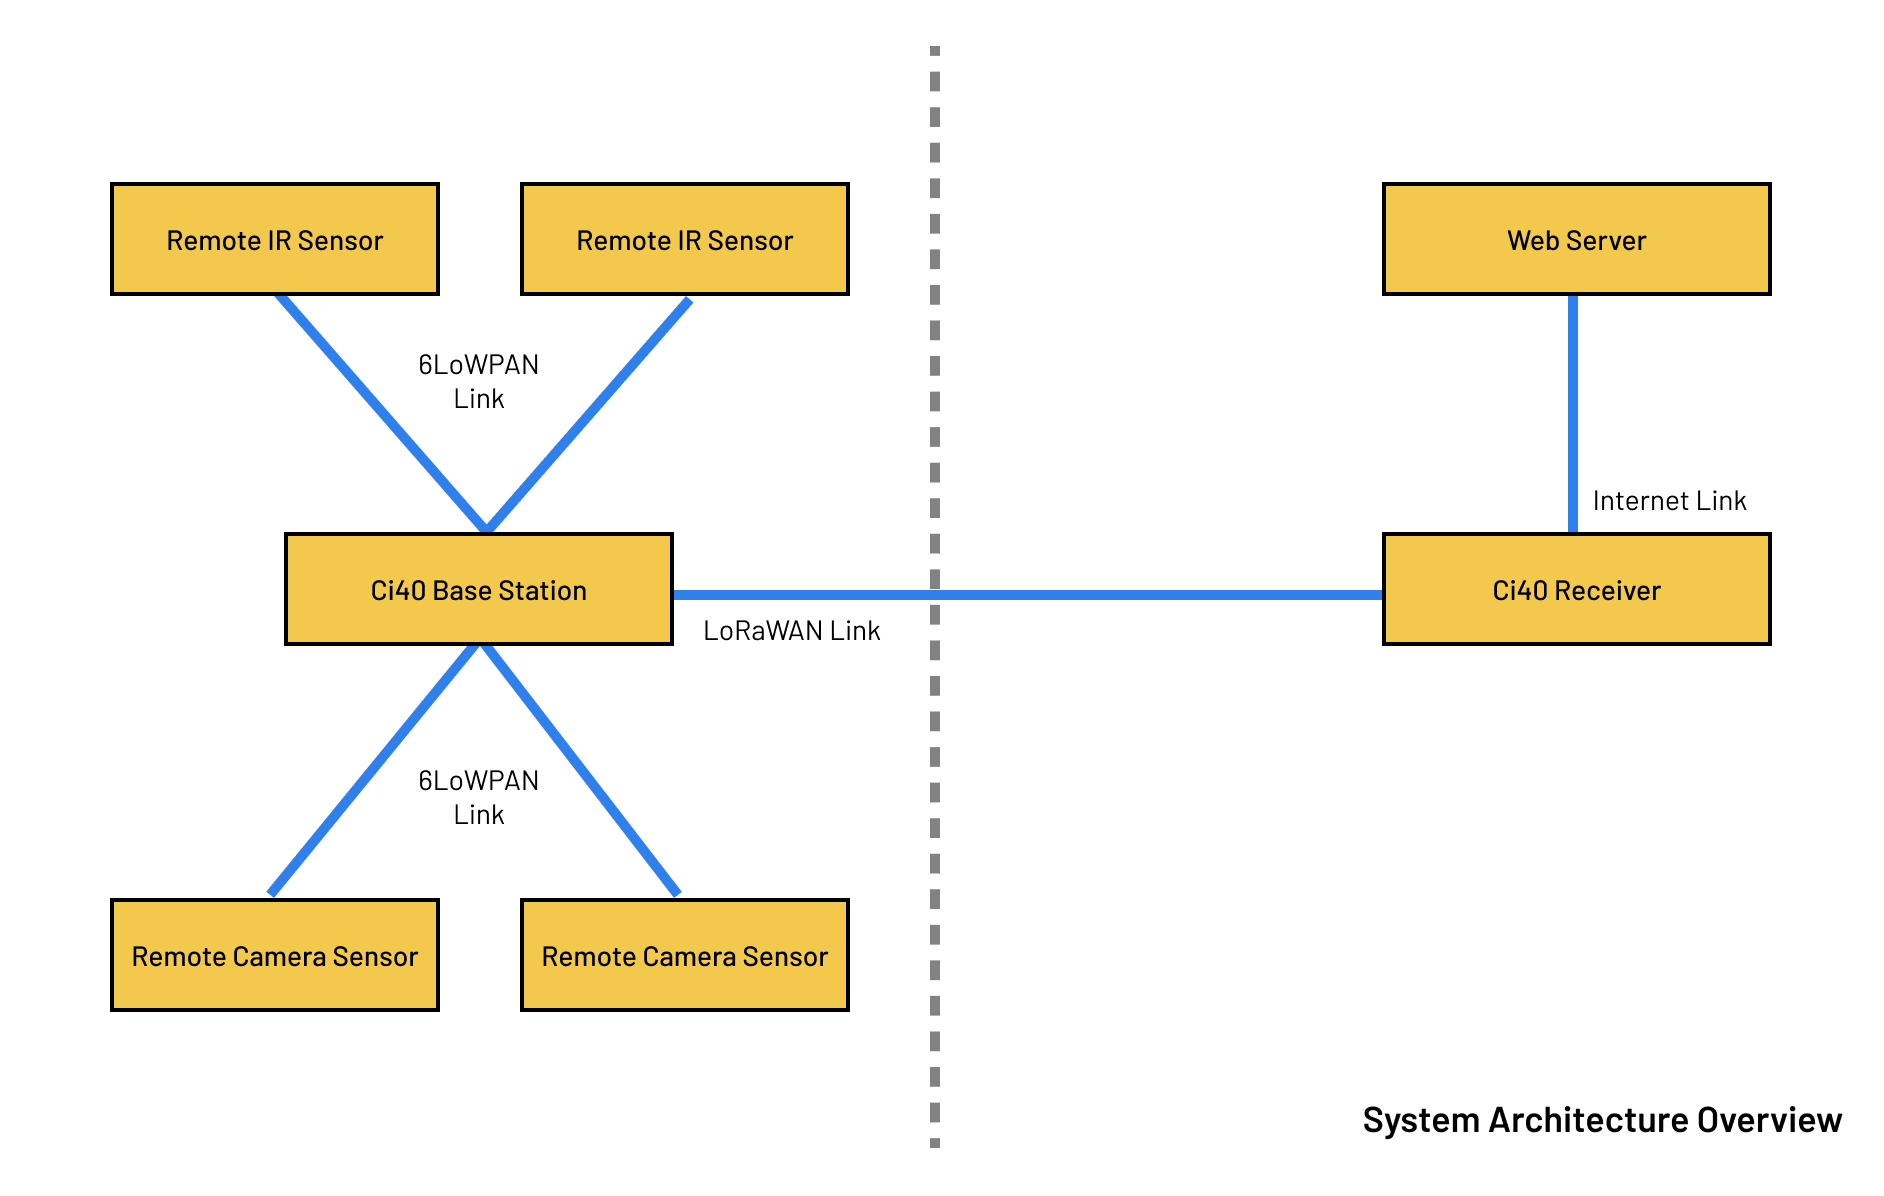
\includegraphics[width=\textwidth]{systemoverview}
  \caption{System architecture overview, showing how the high-level components of the system are connected.}
\end{figure}

Figure~\ref{overviewfigure} shows the connections between the high-level
components in the system, including the sensor deveices and the base
stations, as well as the web server used to store and retrieve data.

\subsection{Base Station}
As previously mentioned in the requirements, the base station is a
\textit{Creator Ci40 \acrshort{iot} Hub} device~\cite{creatorci40}. It is a
development board that is highly specialised for rapidly building
\acrlong{iot} applications, due to its abundance of sockets, pins and radios
for \acrshort{io}.

\subsubsection{Hardware Design Features}

The Ci40 board includes a \gls{6lowpan} radio, which is crucial in allow it
to conduct two-way communication with nearby sensing devices at a reasonably
high data rate. The main drawback is the range, which is typically a couple
of tens of meters~\cite{culler20096lowpan}. However, this is perfect for
communicating with the nearby sensor devices, which won't be too far away
from the base station in the first place, and there is also the potential to
use a mesh-style network, where communication might happen via one or more
intermediary nodes. However, this would require sensor devices to be
constantly active, thus preventing them from entering a lower power state and
resulting in a much higher power usage.

\subsubsection{Software Design}
The base station provides a couple of very important tasks. Firstly, it acts
as the main router, or coordinator, for nearby motion detector and camera
pairs. It receives a motion alert from the motion sensor and sends a command
to the related camera to capture an image. This program would also need to
keep a list of sensor pairs, to ensure each command gets sent to the correct
sensor.

In addition to this, the base station runs a program to process incoming
images from the camera sensors and calculates the count and species of any
wildlife in the photo. Since this is an image recognition problem, it was
decided that the best solution would be to use a convoluted neural network,
trained on a dataset of similar images, to estimate to a reasonable accuracy
the species of wildlife in the image. However, since the Ci40 board uses a
32-bit processor architecture, it makes running neural networks a little more
difficult, since most frameworks will only support 64-bit processors, as the
larger word length results in larger computations being made possible.

Finally, the base station needs to act as a \gls{lorawan} transmitter, to
send the count data to an Internet-connected base station, which can then in
turn upload the results to the web server. So, the base station is running
three programs at the same time to deal with different tasks. All of the code
that deals with the \gls{6lowpan} connection or \gls{lorawan} connection is
written in either C or Python, and uses the \textit{LetMeCreate} library
provided by the board manufacturer to increase ease of development.

\subsection{Remote Sensors}

\unsure[inline]{include graphic of camera pairs in trees etc?}

The system also utilises a set of remote sensors that wirelessly connect with
the base station using a \gls{6lowpan} connection. There's two kinds of
sensors being used in the system, motion detector sensors and camera sensors.
Both sensors use the same base board, a \textit{MikroElektronika}
\gls{6lowpan} Click Board~\cite{mikroeclick}, with either a camera or motion
detector attachment.

\subsubsection{Hardware Design}

\todo[inline]{Include image of 6LoWPAN clicker}
The \textit{MikroElektronika} \gls{6lowpan} Click Board, as previously
mentioned, runs a \acrfull{rtos} called \gls{contiki}. According to the
\gls{contiki} project website~\cite{contiki}, it is ideal for low-power
\acrshort{iot} projects since it supports the full \acrshort{ipv4} and
\acrshort{ipv6} networking suites, as well a being able to run on ``tiny
systems, only having a few kilobytes of memory available''. \textit{Creator},
the manufacturers of the Ci40 base station, provide a toolchain for writing
programs to the click board, as well as abstraction libraries for network and
sensor interfaces~\cite{letmecreate}.

Creator also provide a set of guides to help set up and write programs to the
flash memory onboard the clicker device~\cite{clickersetupguide}, which have
proven invaluable. Code is written in a slightly modified version of the C
programming language; the main difference being that all of the code runs in
process threads that can be suspended, resumed and interrupted.

\subsubsection{Communication}
The remote sensors communicate with the base station using
\acrshort{json}-encoded strings sent via \acrshort{tcp} over \gls{6lowpan}. A
set of commands are defined and recognised by the sensors and the base
station server alike, to allow messages to be sent that are both brief and
human-readable, which is invaluable when debugging. The messages take a form similar to this:

\begin{verbatim}
  { "device_id": 1, "command": "heartbeat" }
\end{verbatim}

A unique \texttt{device\_id} is provided by every sensor to identify itself
to the base station server, and on its first connection it will also provide
a \texttt{pair\_id} which tells the server which unique camera/motion
detector pair the device belongs to. Each of these are provided to the sensor
program at compile time, using environment variables.~\improvement{Add list
of commands?}

\subsubsection{Motion Detector Sensor}
\todo[inline]{include image of motion click}
The motion detector sensor uses the \gls{6lowpan} Click board described
above, with a \textit{MikroElektronika} Motion Click
device~\cite{motionclick} integrated onto the board using the
``\gls{mikrobus}'' port. According to the product page~\cite{motionclick}, it
has a range of up to four metres which is probably not sufficient for real
world usage. However, for prototyping purposes, it is perfect because of the
ease of integration, thanks to the aforementioned \textit{LetMeCreate}
library~\cite{letmecreate}.

The code runs in a continuous loop, that yields the main thread until it is
resumed by an event interrupt. This event could be one of:

\begin{itemize}
  \item a timer expiring,
  \item a \acrshort{tcp} event (received packets, lost connection, et cetera),
  \item a motion detection event received from the motion sensor.\unsure{any
  other events?}
\end{itemize}

For the prototype version of this sensor, the code sends a ``heartbeat''
command to the base station every twenty seconds, for debugging purposes. But
in a production version, the processor would only be be interrupted by
\acrshort{tcp} events or by motion detection events, as this would result in
fewer interrupts over time and thus reduce the power usage of the device. The
development version of the program also makes use of a debug server running
on the base station. The clicker board does not always have a serial
output available, so printing to console (i.e., using the \texttt{printf()}
function) does not work. Therefore, Contiki includes a \texttt{PRINTF} macro
that sends the string to a server using \gls{6lowpan}, if available.

\subsubsection{Camera Sensor}

\todo[inline]{include image of camera click}
The camera sensor comprises of the same \gls{6lowpan} Clicker board, but
instead of a motion sensor, there is a \textit{MikroElektronika} Camera Click
board~\cite{cameraclick} installed onto the \gls{mikrobus} port. The board
contains a digital camera sensor which, according to the specification page,
has a maximum resolution of 640 by 480 pixels. It also contains an extra
microcontroller, which ``outputs the camera image to the target board
microcontroller through the \gls{mikrobus} SPI interface''. Essentially, it
appears to transform the raw data stream from the camera into a data stream
that can be sent using \acrfull{spi} to the `target' board (in this case, the
\gls{6lowpan} clicker). However, a lot of the board's inner
workings\textemdash save for the board schematics, available on the product
page\textemdash is largely closed-source.

The code examples provided by
\textit{MikroElektronika}~\cite{cameraclickexamples} helped to provide a
little bit of insight into how the camera can be operated. For example, it
provides a list of \glspl{opcode} that the camera click accepts, such as
requesting an image, or getting/setting a register on the camera sensor
itself.

The main objective of the camera sensor is to respond to a message sent from
the base station (over \gls{6lowpan}) commanding it to take a photo and send
the photo back to the base station over the same connection.

\subsection{Web Server}
The web server serves the purpose of storing incoming species counts and
types from any number of base stations, as well as keeping track of the
locations of the base stations and sensors. Since the sensors and devices
don't possess geolocation capabilities, this would be something that a
research team using this solution would have to manually input.

As well as providing a way of uploading and storing this information, the web
server would also have to provide methods of retrieving the data, as well as
displaying the data. To this end, an \acrshort{api} is the best solution for
the problem. Appendix~\ref{app:apispec} shows a copy of the \acrshort{api}
specification that was created before development began on the \acrshort{api}
itself. Specifications are highly important, since they could be used to help
develop comprehensive test suites for the code itself, as well as provided a
solid foundation for any further documentation, for instance documentation
that third parties use to build on top of the \acrshort{api}.

The first stage in building the \acrshort{api} is to model how the data is to
be represented. This is achieved in three stages:

\begin{enumerate}
  \item Work out what entities are to be represented with the API. For this
  project, this ended up being: the base stations, the associated sensor
  pairs, and the readings obtained from the sensor pairs. The web server
  doesn't need to concern itself with how the pairs connect to the base
  stations and to each other, so it is easier to model each motion sensor and
  camera sensor as a single pair.
  \item Construct an entity-relationship diagram, to represent how each of
  the entities listed interact with each other. This also introduces the
  notion of multiplicity; for instance, how many base stations does a sensor
  pair interact with?~\todo{include E-R diagram (and ref here)}
  \item For each entity, deciding what data needs to be stored and accessible
  from the \acrshort{api}. As mentioned earlier, a lot of data is actually
  excluded here since it is only relevant at a lower level. An example of
  data that is deliberately excluded is sensor \acrshort{ipv6} addresses,
  since they're only required by the base station for communication. This is
  also when it would be decided what data is necessary and \textbf{must} be
  included for each instance of the entity, and what data is optional.
  Human-readable names are a good example of this.
\end{enumerate}

From this initial requirements gathering, it is then possible to create an
\acrshort{api} specification, detailing how the \acrshort{api} should react
to certain input. It should be highly detailed, included specifying the
\acrshort{http} response code that would be received under normal conditions.

The entire \acrshort{api} specification is included in
Appendix~\ref{app:apispec} for the reader's perusal.
\chapter{Implementation}

It would be very difficult to attempt to build a complete working system
during the course of the project, and that would be wholly out of scope. So
throughout this project, the idea has been to build prototypes that
demonstrate that a fully production-ready solution is viable.

\todo[inline]{Expand on this chapter intro}

\section{Developing The Base Station Code}
The main base station program is just a \acrshort{tcp} server that handles
commands coming in from the camera and motion sensors over the \gls{6lowpan}
connection. Since the Linux kernel can already handle the \gls{6lowpan}
connection, and no other hardware interfaces are required, there was a lot of
flexibility in the choice of language and framework used to build the server.
The Python language ended up being the choice of language, for its ease of
development and pseudocode-like syntax.

The core language library also includes the \texttt{socket} library, which
provides an easy to use, low-level interface for opening and accepting UDP
and \acrshort{tcp} connections. The server has a global dictionary that maps
the id numbers of sensor pairs to the id of a camera sensor and the id of a
motion sensor. This dictionary is populated from sensors which send an
identification (\texttt{id}) command, broadcasting their unique
\texttt{sensor\_id} and their \texttt{pair\_id}. This means that, when a
motion sensor sends a motion detection command to the server, the server can
look up the ID of the camera associated with the motion sensor and send it a
command to capture a photo.

The source code for the base station server is available in section
\ref{code:base-main} \textit{(page \pageref{code:base-main})}.

\subsection{Developing The Species Classification Software}
Less time was available in practice for developing the species classification
software than intended, because of the complications arising from developing
for the remote sensors as well trying to use the camera module. However, some
exploration was made into the the techniques available to detect and classify
species from a photo image.

Naturally, this was a problem well suited for a \acrfull{cnn}.
\acrshort{cnn}s, according to Christopher Olah's blog post on the
subject~\cite{olah2014conv}, ``can be thought of as a kind of neural network
that uses many identical copies of the same neuron''. Each of these `neurons'
uses contains a mathematically trivial function, such as calculating mean
averages of a set of pixel colours, to reduce the problem down. Weighted
values are used to interpret these outputs and produce the final output of
the network. These weights are ``trained'' (adjusted) using a training set of
data, so that the network's output matches the expected output.

\section{Developing The Remote Sensor Code}
The \gls{6lowpan} clicker that the motion and camera sensors use runs on a
\acrfull{rtos} called \textit{Contiki}~\cite{contiki}. The code that runs on
these devices has to be flashed to the onboard flash memory. Therefore,
Creator provide their own toolchain for compiling and flashing user code.
This, however, was extremely difficult to set up, and a lot of time was spent
obtaining the tooling, attempting to install the code, and being able to
access the clicker from my computers. A lot of documentation was missing or
not provided, which made independent investigations into the source code
necessary.

Another issue was with writing the sensor code itself. The only provided
documentation for Contiki is a handful of examples on its source code
repository, as well as a tutorial on the Creator
website~\cite{clickersetupguide}. To complicate matters further, the code
used to program the boards is a modified version of the C language, except
code runs in ``process threads''. However, after a lot of searching on the
web, the Contiki wiki was discovered~\cite{contiki-wiki}. Despite being
incredibly technical, there was helpful pieces of information available there
to help decipher the inner workings of the Contiki platform, notably how the
``protothreads'' work.

Debugging the code was a further complication when developing the sensor
code. The \gls{6lowpan} clicker only has a single MicroUSB port, which is
used for flashing code to the onboard memory, and does not have a USB port of
any kind to connect a serial terminal to. There is only two ways of debugging
the clicker\textemdash{}sending text over the \gls{6lowpan} connection, or
setting the two hardware LEDs on or off. A \acrshort{udp}-based debugging
server is available along with a \texttt{PRINTF} macro, however these did not
appear to work very well, if at all. It was also found that the debugging
server would not work if the device was making a separate connection to the
base station, such as when sending motion commands.

\subsection{6LoWPAN issues}
A reoccurring issue throughout the development of the remote sensors was the
reliability of the \gls{6lowpan} connection. It often took multiple minutes
or more for the remote sensors to connect to the base station, regardless of
whether it was a \acrshort{tcp} connection or a \acrshort{udp} connection.
Sometimes, the devices would not connect at all, and the debugging server
(when it worked) reported multiple dropped messages. Since the Ci40 uses the
2.4 \acrshort{ghz} frequency band, which is shared with many WiFi standards
as well as Bluetooth, there is a possibility that this might be caused by
interference between these devices, especially since all of the testing
environments available during this project were in close proximity to WiFi
links as well as Bluetooth devices, despite best efforts.

A manual published by \textit{NXP Semiconductors} highlights the issues that
can occur from the co-existence of these technologies on the same 2.4
\acrshort{ghz} frequency band~\cite{nxp2013ieee802154coexistence}. Notably,
on page 19, they recommend that ``to achieve satisfactory IEEE 802.15.4
[6LoWPAN] performance in the presence of WLAN interference, a channel
centre-frequency offset of 7 MHz is recommended'', and if \gls{6lowpan} is
running on the same channel as the WiFi link, ``a physical separation from
the WLAN \acrfull{ap} of 8 m is recommended''. Essentially, they recommend
either conducting radio operations away from WiFi \acrshort{ap}, or selecting
a different channel if possible. However, the WiFi \acrshort{ap}s in the
testing environment are managed by a third party, so it was not possible to
change their channels. Additionally, the documentation for the Ci40 base
station was not clear enough on whether it was possible to set the
\gls{6lowpan} wireless channel or not.

As a result of these \gls{6lowpan} issues, some modifications were made to
the project. The camera sensor would be prototyped by installing the camera
module \textit{directly} onto the Ci40 base station, to make development and
debugging easier. Since the Ci40 runs a full Linux operating system and full
WiFi stack, it is possible to connect to it using an \acrfull{ssh}
connection. In addition to this, code designed to run on the camera clicker
was not developed because it would be extremely similar to the motion sensor
code, albeit with the camera processing code instead of the motion sensor
event handling code.

\subsection{Working With The Camera Click Module}
One of the biggest obstacles during the project was working with the
\textit{MikroElektronika Camera Click} module~\cite{cameraclick}, to be used
as part of the prototype hardware for the remote camera sensor. The only
documentation provided for this sensor is available on their ``LibStock''
website~\cite{cameraclickexamples}, but the only documentation provided is a
board schematic and a code example, designed to be used with
\textit{MikroElektronika}'s own TFT display, with its own proprietary image
format.

However, the code example provided was enough to discover roughly how the
camera click board works and responds to input. It uses the \acrshort{spi}
interface to receive commands and send a new or buffered image back to the
parent device. The commands supported are, according to the code examples:

\begin{itemize}
  \item \texttt{\_\_CMD\_WRITE\_REG} (assumed) write to the registers on the
  camera \acrfull{mcu}, to set things like exposure and brightness settings.
  \item \texttt{\_\_CMD\_READ\_REG} (assumed) read from the registers on the
  camera \acrshort{mcu}.
  \item \texttt{\_\_CMD\_GET\_FRAME} capture a new photo and prepare to send
  it back through the \acrshort{spi} interface.
  \item \texttt{\_\_CMD\_GET\_FRAME\_BUFFERED} (assumed) get the currently
  buffered image from the camera, without capturing a new image.
  \item \texttt{\_\_CMD\_SET\_ROW\_NUM} unknown.
  \item \texttt{\_\_CMD\_SET\_ROW\_SIZE} unknown.
\end{itemize}

\subsubsection{The \acrshort{spi} Interface}
The \acrshort{spi} involves one ``master'' device, which sends commands to
one or more ``slave'' devices. There is four data lines involved:

\begin{itemize}
  \item CS\textemdash{}Chip Select. Selects the slave device to use.
  \item MISO\textemdash{}Transmits data from the master device to the slave
  device.
  \item MOSI\textemdash{}Transmits data from the slave device to the master
  device.
  \item CLK\textemdash{}Timing signal.
\end{itemize}

The master and slave devices transmit data as if they were one ``rotary''
system. Each side has a buffer of a fixed size (in the case of the camera
module, 8 bits), and as the master device pushes a bit to the \acrshort{spi}
interface, the slave device sends a bit back. This continues until the
buffers are essentially swapped around.\todo{add SPI diagram} One peculiarity
in this implementation of \acrshort{spi} is that the camera module use sa
separate ``interrupt'' pin (provided by the \gls{mikrobus} standard) to let
the master device know that it is ready for commands.

\subsubsection{Getting Camera Output}
The code in Section~\ref{code:camera-base} shows the code used to attempt to
obtain output from the camera sensor, installed onto one of the Ci40's
\gls{mikrobus} ports. It works by initialising the \acrshort{spi} pins and
setting speed and other settings, before waiting for the camera to send a
``ready'' signal and then sending the \acrshort{spi} command to get an image
from the camera. It then reads the incoming data to a buffer, and saves that
buffer to a file. The data \textit{should}, in theory, be the image data from
the camera. This code should work since it roughly follows the steps used in
\textit{MikroElektronika}'s example code. However, the camera module
frequently returns a lot of blank data. Below is one example of data received
from the camera sensor after sending a \texttt{\_\_CMD\_GET\_FRAME} command:

\begin{verbatim}
  [mbell@chancery-lane ~]$ hexdump ~/out.bin
  0000000 ffff ffff ffff ffff ffff ffff ffff ffff
  *
  000c600 0000 0000 0000 0000 c611               
  000c60a
\end{verbatim}

\subsubsection{Interpreting Camera Output}
Sometimes the camera would send data that was not just a stream of \texttt{1}
bits, however it was not clear whether the returned data was nonsense, or if
the data was in some proprietary data format.

Figure~\ref{fig:yuvimage} shows the data previewed as a \textit{YUV} image.
This is an 8-bit pixel encoded image format that contains three values for
each colour\textemdash{}the brightness (also called luminance), and two
values defining the colour itself (the chroma)~\cite{softpixelyuv}. The data
was estimated to be using some kinda of YUV format, because of reoccurring
patterns in the data that suggested that pixel data was set as some 4-bit
value, then two 2-bit values.

The possibility of the data being stored as \acrfull{rgb} data was ruled out
when attempting to parse the raw image file as such. The results can be seen
in figure~\ref{fig:rgbimage}. It is clear that the data is not \acrshort{rgb}
since the rendering software runs out of bits roughly two-thirds of the way
through parsing the image. Since public access to the source code for the
camera module was prohibited by the manufacturer, it was impossible to tell
whether the image format chosen was incorrect, or if the camera module itself
was defective or damaged. Therefore, no image was ever able to be correctly
obtained from the camera module.

\begin{figure}[h]
  \centering
  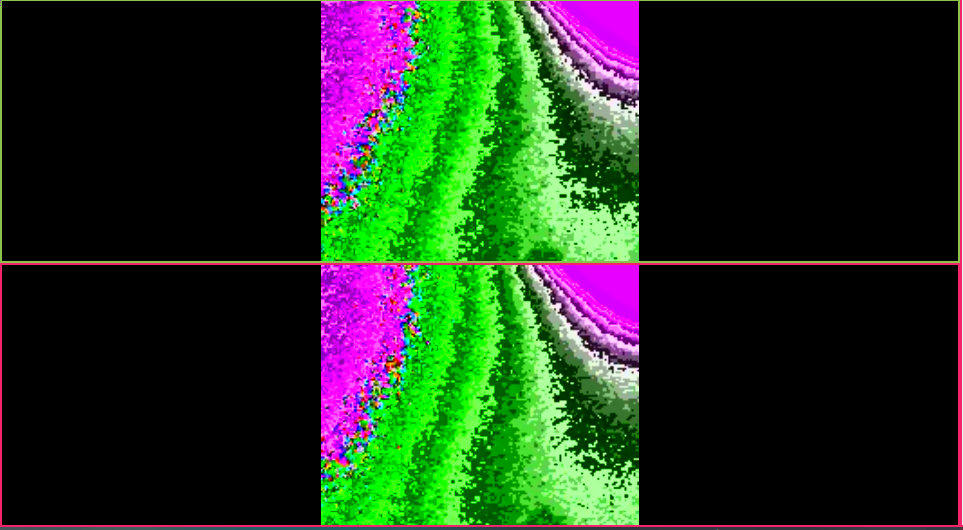
\includegraphics[width=0.8\textwidth]{cameraoutput1}
  \caption{The data received from the camera sensor, interpreted as a
  YUV-formatted image.}
  \label{fig:yuvimage}
\end{figure}

\begin{figure}[h]
  \centering
  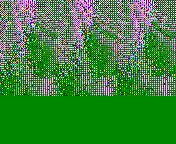
\includegraphics[width=0.8\textwidth]{cameraoutput2}
  \caption{The data received from the camera sensor, interpreted as a
  RGB-formatted raw image.}
  \label{fig:rgbimage}
\end{figure}

\subsubsection{Read-Only Register Random Number Generator}
The camera module used on the camera sensor is the OV7670-VL2A CMOS sensor,
and a datasheet is readily available online~\cite{omnivisiondatasheet}.
Included in the datasheet is a list of the sensor's registers, detailing the
register's:

\begin{itemize}
  \item One byte address (in hexadecimal),
  \item Name of the register,
  \item The default hexadecimal value,
  \item Whether it can be read and/or written to,
  \item And a description of what the register represents.
\end{itemize}

Two of these registers were of significance for testing the \acrshort{spi}
interface, addresses \texttt{1C} and \texttt{1D}. These are both read-only
registers that return the high byte and low byte (respectively) of the two
byte manufacturer ID. They are both read only and are supposed to always
return \texttt{0x7F} and \texttt{0xA2} respectively.

However, when this was attempted on the \texttt{camera\_base} application
(see Section~\ref{code:camera-base} lines 141\textendash{}144), the program
received random numbers each time. \todo{Include screenshot/text output of
command being run} Either one of two explanations is
possible\textemdash{}either the code to read from the register is incorrect,
or the camera click board is defective. As with trying to read the image
itself, it is impossible to conclude which of these explanations is correct
without being able to access the \textit{MikroElektronika} source code.

\chapter{Evaluation and Conclusion}

\section{Evaluation of Expected Deliverables}
Below is a list of the expected outcomes and deliverables specified at the
start of the project and if they have been achieved (and to what extent).

\subsection{Base Station Program}
\textit{``A program built for the Creator Ci40 prototyping board that can
read in an image sent by the external camera module, and classify the types
and counts of animals in the image, before sending this data to a base
station via a LORA connection.''}

\noindent
This deliverable was only partially completed. A small program was created
that can handle sensors connecting to the base station, as well as receiving
motion events, but the classification program was not built.

\subsection{Motion Sensor Program}
\textit{``A program for the IR clicker device to detect movement and send a
message to a nearby camera device.''}

\noindent
This deliverable was completed and works to a reasonable standard, despite
issues with the onboard wireless radios.

\subsection{Camera Sensor Program}
\textit{``A program for the camera device to take a photo when it receives a
command via 6LoWPAN and send it to the Ci40 board.''}

\noindent
This deliverable was not completed, because of multiple issues using the
provided camera sensor and getting any readable data from it.

\subsection{Cloud Server}
\textit{``A simple cloud service to store and display results received from the
prototype boards''.}

\noindent
This deliverable was completed to a high standard.

\subsection{Tests}
\textit{``A rigorous testing regime for as much code as possible.''}

\noindent
This deliverable was met for the cloud server, as well as acceptance testing being conducted for the motion sensor.

\subsection{Real-Life Test}
\textit{``(If possible) a real-life test of the system in an uncontrolled
environment (i.e. a park or zoo).''}

\noindent
This was not met due to the other incomplete deliverables.

\section{Evaluation of Achievements}
Despite not all goals being met, the project should overall be considered
successful. The research conducted early in the project highlighted a clear
need for such an autonomous system to be developed, and recent strides in the
field of computer vision mean that such systems are becoming faster and
cheaper to deploy. However, it was a shame that not all of the deliverables
could be completed, especially being able to test the system in a real-life
setting.

One of the biggest and persistent issues throughout the project was problems
developing on the given hardware and using it to the best of its ability.
These problems were discussed in the \textit{Implementation} chapter,
including lack of documentation regarding the libraries used to connect to
sensor and hardware, as well as wireless connections not working as intended.
In hindsight, perhaps it would have been best to swap the hardware out for
better documented, more reliable (although perhaps a lot less realistic)
hardware, like the Arduino platform~\cite{arduino}. The devices may not be as
energy efficient as the ones used in this project, but that could be
considered a less important characteristic for a technical demonstration.

Also, it may have been wiser to begin researching and developing the deep
learning classifier earlier on in the project. The work plan, devised at the
start of the project, mentioned researching and developing this section of
the project from November onwards, whereas perhaps research into different
techniques and frameworks should have been made earlier on.

\section{Possible Future Work}
There is a lot of promise in developing deep learning solutions to such a
problem as automatically classifing animals in camera trap images, and a lot
of recent breakthroughs have been extremely exciting\textemdash{}including
the work of Elias et al~\cite{elias2017s} whose work was published since the
start of this project. Perhaps the rise of general yet powerful models for
computer vision such as Inception-v3~\cite{szegedy2016rethinking} remove most
of the need for bespoke models to be created to solve these kinds of
problems, allowing more and more people to build exciting and powerful
applications for computer vision classification.

Additionally, leaps in the field of mobile computing are also incredibly
exciting. New development boards are appearing every day that can run on very
small amounts of power, vastly increasing expected lifetimes of such projects
as this one, as well as reducing costs needed to maintain and replace
sensors; perhaps future work in this domain could include building clustered
networks of sensors that can be highly resilient to link disruption, yet
still consume just a small amount of power.

\nocite{*}

\renewcommand{\chaptername}{Appendix}
\appendix

\chapter{Glossaries}
\glossarystyle{listgroup}
\printglossaries

\chapter{Bibliography}
\printbibliography[heading=bibempty]

\chapter{Code Listing}

\section{base/\_\_main\_\_.py}
\inputminted[linenos]{python}{../base/__main__.py}

\section{detect/detect.c}
\inputminted[linenos]{C}{../detect/detect.c}

\section{classify/classify\_image.c}
\inputminted[linenos]{python}{../classify/classify_image.py}

\end{document}

